%%%%%%%%%%%%%%%%%%
%  placeholders  %
%%%%%%%%%%%%%%%%%%
\documentclass[9pt,book]{IEEEtran}


\newcommand{\uni}{Technical University of Munich}
\newcommand{\department}{TUM Department of Informatics}
\newcommand{\chair}{Chair for Applied Software Engineering}
\newcommand{\city}{Munich}
\newcommand{\country}{Germany}

% TODO: Replace with your information
\title{ML-Approach to reduce the Optimism Bias towards Climate Change}
\newcommand{\authorname}{Andreas Binder}
\newcommand{\email}{andreasjosef.binder@tum.de}

%\documentclass[conference]{IEEEtran}
\IEEEoverridecommandlockouts
% The preceding line is only needed to identify funding in the first footnote. If that is unneeded, please comment it out.
\usepackage{cite}
\usepackage{amsmath,amssymb,amsfonts}
\usepackage{algorithmic}
\usepackage{graphicx}
\usepackage{textcomp}
\usepackage{subcaption}
\raggedbottom
\usepackage{xcolor}
\def\BibTeX{{\rm B\kern-.05em{\sc i\kern-.025em b}\kern-.08em
    T\kern-.1667em\lower.7ex\hbox{E}\kern-.125emX}}
    
\begin{document}

\author{
	\IEEEauthorblockN{\authorname}\\
	\IEEEauthorblockA{\textit{\department, \chair} \\
	\textit{\uni}\\
	\city, \country \\
	\email}}

\maketitle

\begin{abstract}
Most people believe that climate change is in some way happening. More importantly, many people are convinced that it will have tremendous consequences for the current generation as well as for those yet to come. Although it is common knowledge that changes are going on, there are just few that take action. As the human race is not self-destructive in its self, this inactivity might be explained by the Optimism Bias. In short, people feel affected by threats that seem more impending to them privately. This fosters the believe that catastrophic events like bushfires in Australia are being far away from them and therefore making them less concerned. We want to overcome that bias by utilizing Machine Learning. To do so, our work is inspired by the contributions of Viktor Schmidt et. al. who implemented a Cycle-Consistent Generative Adversarial Network to predict how a house might look like after being hit by a flood. Our eventual goal now is to be able to take pictures of a house as an input and then create an image of the same house burning. The data is self collected, and the trained model currently only aims to generate pictures of burning houses. Our work should help people to envision possible future scenarios for their home and hence could lead to a stronger incentive to actively fight climate change.  
\end{abstract}

%%%%%%%%%%%%%%%%%%%%%%%%%
%  General Information  %
%%%%%%%%%%%%%%%%%%%%%%%%%

% Keep the slides from the Kick-Off Meeting in mind.
% The goal of the seminar is to take a look at applications of machine learning in real world scenarios or with real world applications.
% We want to take theoretical concepts and new approaches and apply them to existing or emerging problems.
% It is important that you document your process, collect citations, the process how you got to the results is as valuable as the end result.
% The seminar be about 6 pages (+ bibliography) long. It should summarize your literature research and related work.
% - Related practical work e.g. frameworks, tools, applications
% - Related academic literature such as papers and books
% - Showcases your proposed solution and prototype
% - Describe the implementation, challenges, and interesting technical details
% - Showcase why your prototype is a relevant for consumers or research
% - Details possible future work

\section{Introduction}
    \subsection{Motivation}\label{Motivation}
    %Tell the reader about my plan
	In this paper we want to illustrate the impact of climate change through visual transformations using Generative Adversarial Networks (GANs). 
	%what is it all about
	Tackling the climate crisis is one of the most urgent issues in this century\footnote{https://www.un.org/en/sections/issues-depth/climate-change/}. Countermeasures are complex and demand the cooperation between nations, businesses and cultures. Hence, the more important it is that everyone pulls together\footnote{https://www.un.org/sustainabledevelopment/climate-change/}. Nevertheless, there are many people who are not aware of the dimensions of climate change or even deliberately deny them or, in the worst case, accelerate climate change. \\
	Admittedly, most people only notice those consequences directly that are not yet threatening, such as rising temperatures. Because of this, an average person cannot yet deduce the final intensity that might follow. The Optimism Bias\footnote{https://en.wikipedia.org/wiki/Optimism\_bias} is the key word here that makes many people think that everything changes again for the positive or that they are not affected.
	Even pictures of catastrophes such as floods or melting icebergs appear far away and not harmful. Some have the pictures in the back of their minds, but those vanish again during their everyday life. \\
	The lack of psychological affection\cite{behavioural} is the gap we want to close. In this report, we would like to focus on houses that were set on fire by a forest fire, a typical consequence of climate change.
	%how do I do it 
	We would like to take action against the presented misjudgments by showing the deniers which effects climate change can have on them, and in this case their house. This work is intended to be the cornerstone for a longer project. To be precise, we create a model that does not create real, but realistic looking images from a lot of pictures of burning houses as the first step.\\
    
\section{Related Work}
\subsection{Generative Adversarial Networks}
    There exist a great deal of generative neural networks, for example Deep Boltzmann Machines, Variational Autoencoders and Generative Adversarial Networks, to name just a few. Nevertheless, the latter has to have something to it, since it has gotten a lot of hype recently and was even described by Yan LeCun as "the coolest idea in machine learning in the last 20 years"\footnote{https://www.youtube.com/watch?v=IbjF5VjniVE}. GANs have many use cases, including encryption, data manipulation and testing of security systems. However, the most popular use case is the generation of images.
    
\subsection{How does a GAN work}
	%how does a GAN work
	For this task of image generation, we make use of Generative Adversarial Networks. A GAN belongs to the class of the generative neural networks. GANs consist of two deep neural networks, commonly called Generator and Discriminator with respect to their adversarial task. They are trained by playing a min-max zero sum game where each loss is depending on the actions of the other network. The Generator maps a probability distribution to a visual output in form of multi-dimensional tensor. The Discriminator on the other hand provides feedback on the multi-dimensional output of the Generator by mapping it back to a probability distribution. \\
	
	\begin{figure}[htb] 
    	\centering
    	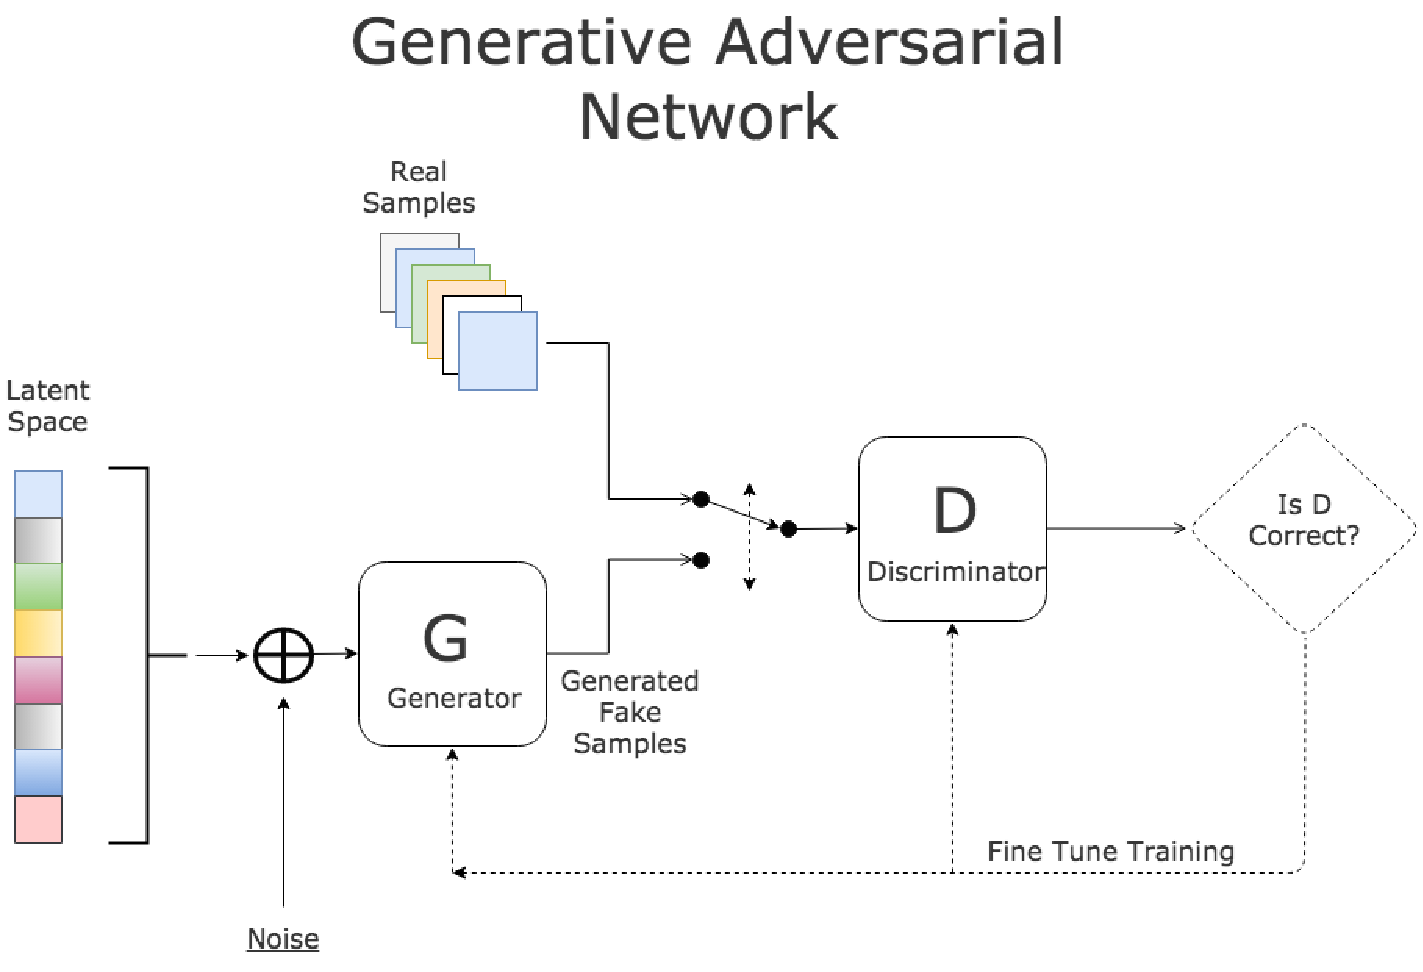
\includegraphics[width=0.7\linewidth]{GAN_structure.pdf}
    	\caption{Discriminator and Generator in the context of GANs}
    	\label{fig:GAN}
    \end{figure}
	\footnote{https://medium.com/ai-society/gans-from-scratch-1-a-deep-introduction-with-code-in-pytorch-and-tensorflow-cb03cdcdba0f}
	
	Hereby, the Discriminator assigns probabilities to each class the generated image might belong to. As we consider a binary decision between 0 and 1, the final layer of the Discriminator will be a single neuron. The Generator does not have direct access to the real data that it should eventually be able to create instances of, but the Discriminator does as he is fed with fabricated input from the Generator and real samples. Hence, the Discriminator tells the Generator about the quality of the learnt features indirectly through its loss function. By iteratively incorporating the provided feedback the Generator will ultimately produce outputs that the Discriminator cannot distinguish from the real samples which leads to the Discriminator outputting a probability of 0.5 for any generated image created by the Generator.  
    %who started this idea
    GANs were first introduced by Ian Goodfellow \cite{goodfellow2014generative} in 2014. The Generator G tries to minimize the value while the Discriminator D tries to maximize it. The formula depicting this behaviour looks as follows: 

    \begin{equation}
        \min_{D} \min_{G} V(D,G) = \mathbb{E}_{x \sim p_\textbf{data}(x)}[\log D(x)] + \mathbb{E}_{z \sim p_\textbf{z}(z)}[1-\log D(G(z))]
    \end{equation}
    
\subsection{Unpaired Image-to-Image Translation}
    At the end of 2018, Jun-Yan Zhu et al. published an authoritative paper dealing with unpaired image to image translation \cite{zhu2017unpaired}.
    In this paper, image to image translation is defined as follows: image-to-image translation is a class of vision and graphics problems where the goal is to learn the mapping between an input image and an output image using a training set of aligned image pairs.\\
    This implies having paired image data, since images of the same object are required by the source and the target domains. This confronts us with the problem of data availability. In many areas, collecting images in pairs is either extremely difficult (images of houses before flooding) or even impossible (in the case of deceased artists who obviously will not draw new paintings that you could use).\\
    Therefore, Jun-Yan Zhu et al. introduce an extension of the Generative Adversarial Network, namely the Cycle-Consistent GAN. With the help of a consistency loss an attempt is made to increase the quality of the images. Given are two projections G: X$\,\to\,$Y and F: Y$\,\to\,$X, where X and Y represent domains. For an input x the loss is calculated from the difference between x and F (G (x)) and thus minimizing the loss will result in more accurate and vivid representation of the observable world.\\
    The use of two mappings instead of one and the introduction of the cycle consistency loss is the main difference to a standard GAN. Since we map bidirectionally between domains, we need two additional loss functions, one for the forward cycle consistency and one for the backward cycle consistency:
    
    \begin{multline}
                \L_{cyc}(G,F) =  
        \mathbb{E}_{x \sim p_\textbf{data}(x)}
        [ \lVert F(G(x)) - x \rVert_{1} ] + \\
        \mathbb{E}_{y \sim p_\textbf{data}(y)}
        [ \lVert F(G(y)) - y \rVert_{1} ]
    \end{multline}
    
        
    \subsection{Visualizing Climate Change}
        If you research CCGAN, you will primarily get to see beautifully fabricated images of winter landscapes or fails that happen when horses are transformed into zebras. Viktor Schmidt et al. \cite{schmidt2019visualizing} present another interesting approach in this year's paper, which is intended to illustrate the dimensions of climate change to people.\\
        Using climate predictions, they tried to realistically represent the effects that would occur within 50 years. They initially limited themselves to a flooding scenario, i.e. simulating houses in the event of inundation. However, their declared goal is to extend the forecast to other domains later on. Nevertheless, this scenario alone is already relatively intricate. Since there is no database with pictures for such a case, they were searched manually on the web. In addition, only images with almost no external factors have proven useful. Their dataset consists of detached houses with a garden or greenspace in the foreground. \\
        Their work eventually got our interest and made us initiate the project we will describe in the following sections.
\section{Contributions}
\\
In this section, we will provide an overview over the data set, the training structure, the network architecture, the hyperparameters and the used evaluation techniques. We will also briefly describe our prototype.  

    \subsection{Dataset}

    Currently, the dataset consists of 329 colored pictures with a mean size of 828X1244 which is pretty big compared to the resized training data. This particulary large gap is one of the problems that arose while training. The pictures are self-collected, mainly by browsing the web. Subjectively, the results from the search engine duckduckgo.com were superior to the one suggested by google.com or startpage.com since it offered are more accurate results when searching for key phrases in this specific context. \newline
    The most pictures were found when seeking for burning houses in California. Since the wildfires in California are caused by the effects of climate change, the relation is sound. \newline
    Additionally, a big chunk of pictures came from the recent bushfires in Australia. The rest of the images do not have a connection to a specific event. Most houses are wooden and are surrounded by trees and dry areas. Similar to Schmidt et al.\cite{schmidt2019visualizing}, we tried to avoid images with extraneous features to prevent many-to-many mappings. Also the brightness of the pictures is also quite intense on average what is caused by the blaze and which makes the fire the dominant feature. For retrieving the data from the storage directory and for the different kinds of data augmentation we used the PIL library. It offers a broad range of tools from which we used flipping, cropping, rotating and sharpening. Except for the singular flipping, each augmentation method was applied at least twice with varying parameters. Eventually, we ended up with around 3619 pictures usable for the training of the model.\\
    Beforehand, we resized the pictures to 300X300 pixel which were then later adjusted as well for the sake of comparing the outcome. The sizes we tried have a range from 50 to 250 pixels.\\
    The optimal size lays between 100 and 200 pixels because within that range it is possible to find features on the generated pictures without having to deal with matrix multiplications of enormous size.
    For a small fraction of tasks, as the conversion of the numpy array back to the image, we used functions provided by the Keras API for image processing.
    
    \subsection{Training Structure}
    Concerning the implementation of the network, we first looked at the code written by Ivan Vasilev, proposed in his book "Python Deep Learning" \cite{PythonDeepLearning} in the Chapter about Generative Models. Hereby, we followed his training procedure, however the rest was adjusted according to our project's needs. Because our dataset cannot be imported with being ready for use, an infrastructure for loading as well as for the conversion to multi-dimensional tensors became necessary.\\
    Additionally, the loading of previously saved models and the saving of pictures and of the Generator itself can be customized. Lastly, we included the possibility to evaluate the model performance via Inception Score.
    
    \subsection{Network Architecture}
    We tried different compositions of layers, all of which deliver different results. First of all, we would like to present the heuristics that we found useful and that are backed up by theory. \\
    
    \subsubsection{Batch Normalization}
    The first enhancement applied is Batch Normalization which was developed by Serge Ioffe et al. and presented in their paper "Batch Normalization: Accelerating Deep Network Training by Reducing Internal Covariate Shift" \cite{ioffe2015batch} in 2015. Batch Normalization normalizes every minibatch, so it is possible to decide for each layer individually whether you want to use Batch Normalization. It works by standardizing the output of the activation function. The result is then multiplied by an arbitrary value gamma and added to another arbitrary value beta. In general, this improvement is meant to speed up the training process as well as eliminate unbalanced weights. In our case, after 10000 to 15000 epochs, we came to comparable results that we had previously received after 15000 to 20000 iterations. While conducting research, we found contradicting suggestions, some using Batch Normalization before applying the activation functions and some do it afterwards. Since we am not working on a model that is too complicated, we did not notice any sizeable differences when we chose between these two options.
    \\
    \subsubsection{Normal Distribution}
    \\
    As soon as the model is trained, it can make more or less meaningful predictions. In order to do so, the generator needs an input that it should transform for a prediction, which can be executed in form of the normal distribution or the uniform distribution. In most sources we saw the normal distribution as the standard where the input was taken from. As far as we know, there is no reason backing up this decision, in the end it is up to personal preference. We also did not notice any discrepancies in some small tests we performed. 
 
    \subsubsection{Leaky Relu}
    There are many problems that can arise when training neural networks, one of which is the vanishing gradient problem. The gradient then takes on such a small value that the weight practically does not change. If many neurons are affected, this can prevent the network from learning. \newline
    Therefore, the rectified linear unit (ReLU) is preferably used over sigmoid, because the latter one suffers from the vanishing gradient problem. ReLU, on the other hand, can set the update of the neuron weight to 0 since it only allows 1 for positive values and 0 for negative ones with respect to its derivative. Hence, some neurons may basically die with the consequence that a big part of the network may become untrainable.
    Leaky ReLU counters this effect by returning small negative values for inputs x < 0 which resolves the issue of dead neurons. 
    
    \begin{figure}[htb] 
    	\centering
    	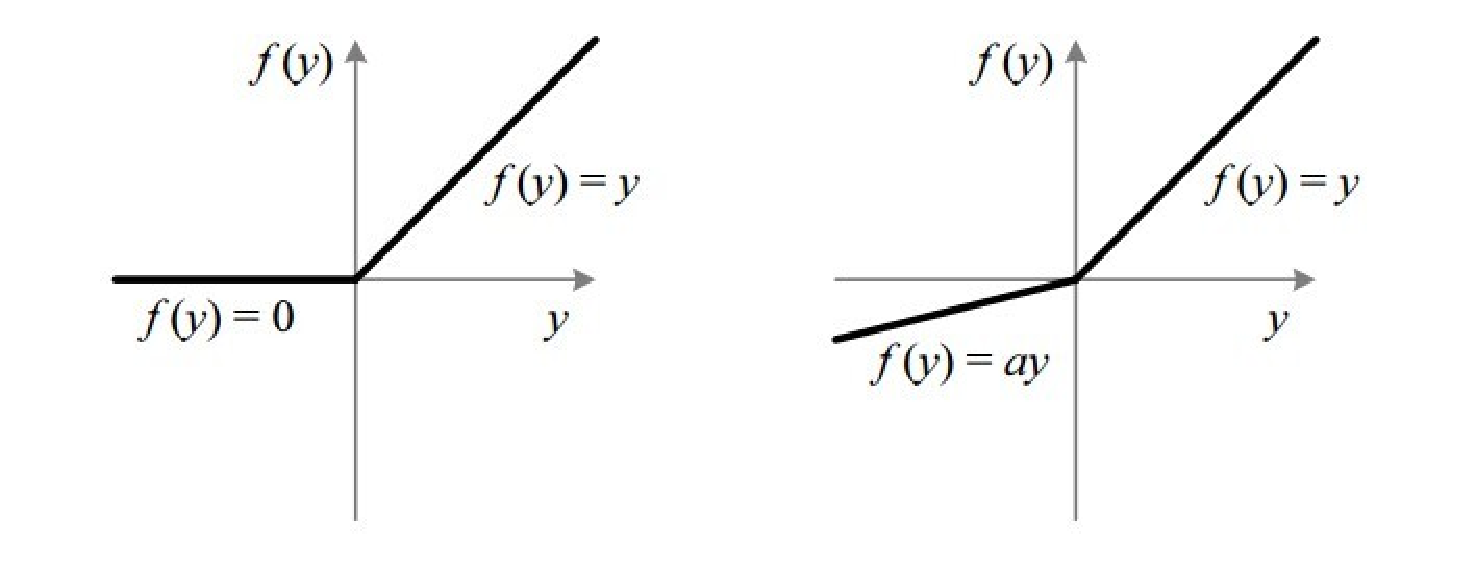
\includegraphics[width=1.0\linewidth]{Relu.pdf}
    	\caption{Comparision between ReLU (left) and Leaky ReLU (right)}
    	\label{fig:Relu}
    \end{figure}
	\footnote{https://towardsdatascience.com/activation-functions-neural-networks-1cbd9f8d91d6}
    
    
    
    \subsubsection{Dropout}
    Dropout is one of the newest but also most effective regularization techniques. It is a layer that accepts the dropout fraction as a parameter. It ranges from 0 to 1 and specifies the percentage of how many output features should be set to 0. \\
    Although at first glance, it may not be entirely clear how this contributes to the stability of the network, once you think about it it is actually conclusive. With this technique it is possible to break up conspiracies, as it is called by  the inventor Geoff Hinton\cite{JMLR:v15:srivastava14a}. In the end you want to force the network to form a robust representation of the input. This is done through introducing redundancy. By preventing the formation of insignificant patterns, overfitting can be tackled. By using dropout, especially at the end of the discriminator, we definitely could get better results over all.

    \subsection{Hyperparameters}

    We already discussed activation functions, specifically the usage of Leaky ReLU, already, nonetheless we want to point out an exception to that heuristic. Specifically, for original GANs it is accepted as standard to use a bounded activation function for the last layer of the Generator. Radford et al. \cite{radford2015unsupervised} argue that the model may "learn more quickly to saturate and cover space of the distribution" when going for a bounded activation function. We opted for tanh, sigmoid would be also a possible alternative. This rule, so to speak, is not true for extensions of the original GANs, like the Wasserstein GAN\cite{arjovsky2017wasserstein} which we cover later because it applies a linear activation function to its last layer of the Generator. Since GAN training is generally considered to be unstable, we tried to stick to prevalent conventions when choosing hyper parameters. \\
    We took Adam as optimizer which we preferred over RMSprop. We changed the learning rate in an interval from 0.0001 to 0.0004, with 0.0002 returning the best results. If the values are set too high, lets say 0.005, there was only a strong red or yellow tone recognizable on the pictures, without the possibility of interpreting other features. The Discriminator and the Generator both implemented the Adam optimizer with the same parameters, the same applies to the loss function, where we used binary crossentropy. \\
    With respect to the Discriminator, the choice definitely makes sense since binary crossentropy is designed for yes or no decisions. We cannot make judgements about the Generator however, first we would like to further adjust other hyperparameters and the network architecture before we experiment with the loss function.\\
    Finally, the samples we submitted to our testers were trained with between 9000 to 17000 epochs.

    \subsection{Evalution}

    There is no standard for Generative Adversarial Networks to evaluate the generated outcome. We therefore decided to use a mathematical evaluation method and the intuitive approach, namely by asking human inspectors for feedback. 

    \subsection{Inception Score}
    One wants to take two ideas into account when calculating the Inception Score. On one hand, that the individual image is highly meaningful (little entropy), on the other hand, that the images are as different as possible from one another. Two distributions are included for this evaluation. The label distribution returns a high value if the generated image could be clearly classified in a target category. The marginal distribution is optimally evenly distributed since all target classes should be served by the model if possible. Ultimately, these two distributions must be compared, for which the Kullback – Leibler divergence is used. If two unequal distributions are compared, a high value is calculated. The more dissimilar these distributions are, the higher the number will be, which is why a higher Inception Score is desirable. Let us consider the example of mode collapse in which the same image or a slight variation of it is produced regardless of the input. Since this is usually an image of higher quality, we receive a narrow label distribution. However, because there is little to no diversity among the generated images, the marginal distribution is also narrow. Due to the proximity of the two distributions, this leads to a low Inception Score. Finally we take the exponential of the result to increase the expressiveness of the number. We used the calculation of the score from this article. \footnote{https://machinelearningmastery.com/how-to-implement-the-inception-score-from-scratch-for-evaluating-generated-images/}Unfortunately, in most cases the Inception Score was not very meaningful for several reasons. The example of mode collapse at times occurred. In addition, our domain (burning houses, most of them wooden) is not directly represented in ImageNet database\footnote{http://www.image-net.org/}, from which the underlying Inception Classifier draws its classes, only boats houses or restaurants for example are available. Fire, the main feature of our dataset, is not present there either. Therefore, regardless of whether pictures were viewed by friends or by ourselves as of good quality, pictures received a low inception score or the same as pictures that we rated as of poor quality. We repeated this inspection process 10 times with 100 images per bad / good generator.

    \subsection{Judgement by Human Supervisor}

    Since the Inception Score did not turn out as applicable in this case, we primary had to rely on human judgement. On one hand, this makes sense, of course, since the image generated is ultimately intended for the human eye which can quickly discover any discrepancies to the real object or scene, given those differences are not too fine. Even if the accuracy of the checking of single images is more or less assured, the tester cannot check a large amount of samples, which is necessary for large networks with many output classes. As also mentioned by Ian Goodfellow in his book "Deep Learning" \cite{Goodfellow-et-al-2016}, humans are not able to find the lack of variation for a huge number of generated images. Luckily, our model is a less intricate one with only one output class. Whether the model has successfully learned the distribution is therefore a yes or no question. To get feedback, we kept putting pictures in a designated folder in google drive which we made accessible to the testers. We have set the test size to 100 pictures, because this gives more information about the average quality of the pictures. Nevertheless, it is still a reasonable size before the testers lose their motivation et cetera. The test subjects worked unpaid, which is why the task was performed by a group of friends of us. When presenting the pictures, however, we told half of the inspectors what they are expected to see in the pictures and for the other half we left room for interpretation. In the group without specifications, the answers were very wide-ranging, occasionally people tapped on fire due to the many shades of yellow and red. Houses or even burning houses could not be recognized. The instructed control group was able to detect the fire quite reliably, although the quality description still fluctuated greatly. In some of the pictures, outlines of houses could already be seen. Intuitively, of course it makes little sense to train the subjects to look for certain features. In the end, this should be done without outside help. Nevertheless, we were able to evaluate the quality of the individual features, in this case primarily fire, even if the overall picture of house plus fire plus environment is still quite vague. Overall, we are very satisfied with our testers. If we had used crowd-sourcing platforms, we would have had similar problems regarding motivation or concerning the set-up.

    \subsection{Prototype}
    We do not want to force everyone who wants to see the results of our project to download and run the code. We are of course happy about feedback, but we would also like to address people without a programming background. Therefore a prototype is available on our homepage \footnote{https://home.in.tum.de/~bindera/}. The model on that page was transformed from python to tensorflowjs using the provided tensorflowjs converter. We tried to keep the design and the code fairly clear. When you go to the page, you are only asked to enter the number of images to be generated. The required logic is completely written inside the index.html file. The styling takes place there as well.


\section{Results \& Discussion}

    In this section, I show some of our results and point out problems that occurred. The presented pictures are mostly of size 200X200.
    \subsection{Results after 7500 Epochs}\\
    After 7500 epochs, sometimes the outlines of houses are recognizable. Bright spots that might indicate a fire are partially set correctly. The brightness and intensity of the fire is relatively low. Example 1 and Example 2 can be interpreted as burning houses at night time.

    \begin{figure}[htb!] 
    	\centering
    	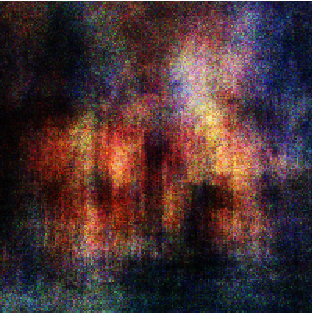
\includegraphics[width=0.7\linewidth]{7500-1.pdf}
    	\caption{Example 1: Door and Windows recognizable}
    	\label{fig:7500-1}
    \end{figure}
    
    %\pagebreak

    \begin{figure}[htb!] 
    	\centering
    	
\includegraphics[width=0.7\linewidth]{7500-2.pdf}
    	\caption{Example 2: Double Pitch Roof}
    	\label{fig:7500-2}
    \end{figure}

    \begin{figure}[htb!] 
    	\centering
    	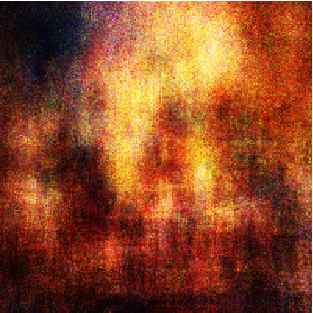
\includegraphics[width=0.7\linewidth]{7500-3.pdf}
    	\caption{Example 3: Mix of Example 1 and 2}
    	\label{fig:7500-3}
    \end{figure}
    
    \pagebreak
   
    \subsection{Results after 10000 Epochs}\\
        At around 10000 epochs, the fire reaches the desired intensity. The outlines that could be interpreted as houses are slowly disappearing.
    
    \begin{figure}[htb!] 
    	\centering
    	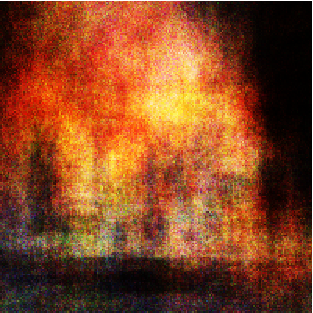
\includegraphics[width=0.7\linewidth]{10000-1.pdf}
    	\caption{Example 4: Fire in House Shape}
    	\label{fig:10000-1}
    \end{figure}

    \begin{figure}[htb!] 
    	\centering
    	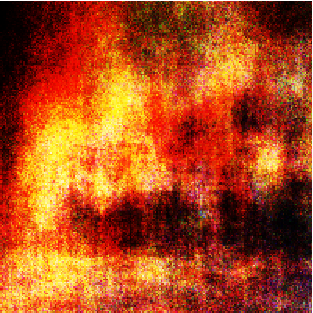
\includegraphics[width=0.7\linewidth]{10000-2.pdf}
    	\caption{Example 5: Windows discernable}
    	\label{fig:10000-2}
    \end{figure}

    \begin{figure}[htb!] 
    	\centering
    	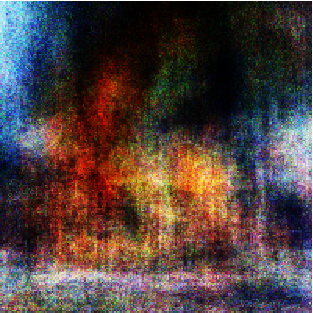
\includegraphics[width=0.7\linewidth]{10000-3.pdf}
    	\caption{Example 6: House with Smoke on Top}
    	\label{fig:10000-2}
    \end{figure}


    \subsection{Results after 15500 Epochs}\\    
    The picture becomes a mixture of yellow, red and black sections. It will overlap the point to see anything other than fire. The red tones might even be interpreted as lava.

    \begin{figure}[htb!] 
    	\centering
    	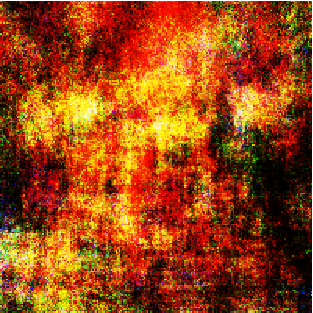
\includegraphics[width=0.7\linewidth]{15500-1.pdf}
    	\caption{Example 7}
    	\label{fig:15500-1}
    \end{figure}    

    \begin{figure}[htb!] 
    	\centering
    	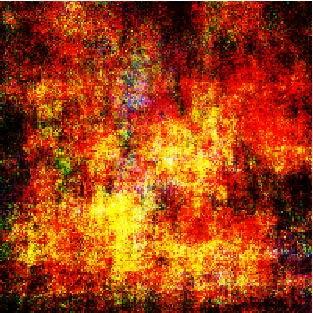
\includegraphics[width=0.7\linewidth]{15500-2.pdf}
    	\caption{Example 8}
    	\label{fig:15500-2}
    \end{figure} 

    \begin{figure}[htb!] 
    	\centering
    	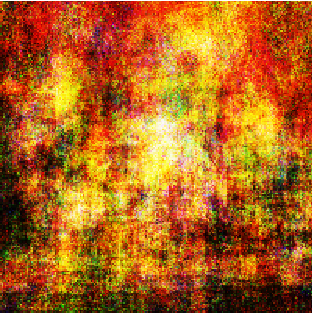
\includegraphics[width=0.7\linewidth]{15500-3.pdf}
    	\caption{Example 9}
    	\label{fig:15500-3}
    \end{figure} 

    \subsection{More Examples}\\
    Those pictures are of smaller size, 75X75 to be precise, after 10000 epochs. \\
    \begin{figure}[htb!]
    \centering
        \begin{subfigure}[htb!]{0.3\linewidth}
        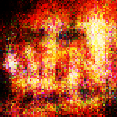
\includegraphics[width=\linewidth]{10000-1(7575).pdf}
        \caption{}
        \end{subfigure}
        \begin{subfigure}[htb!]{0.3\linewidth}
        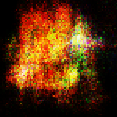
\includegraphics[width=\linewidth]{10000-2(7575).pdf}
        \caption{}
        \end{subfigure}
        \begin{subfigure}[htb!]{0.3\linewidth}
        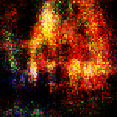
\includegraphics[width=\linewidth]{10000-3(7575).pdf}
        \caption{}
        \end{subfigure}
        \begin{subfigure}[htb!]{0.3\linewidth}
        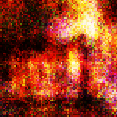
\includegraphics[width=\linewidth]{10000-4(7575).pdf}
        \caption{}
        \end{subfigure}
        \caption{Samples with 75X75 pixels.}
        \label{fig:coffee3}
    \end{figure}


\subsection{Problems}
\\
Unfortunately, fire is by far the most dominant feature in our dataset. In addition, the structure of the second important feature, the houses, is more difficult to recognize because it is composed of several more complex features. While in the case of fire, basically only the transition from yellow to red areas has to be learned, a house has significantly more criteria to go through as such. This includes vertical side walls, windows, in most cases tapered roofs, etc. In addition, resizing means that even more meaningfulness disappears because fine structures can no longer be perceived because they blur. This problem could be seen as a kind of mode collapse based initiated by the Discriminator. Mode collapse normally means that the Generator specializes itself mapping only one distribution, for example that of cats, since those images previously have been successfully accepted, even though dogs are also included in the data set. In our case the quality of the houses is not sufficient so that the Discriminator fails to incorporate this feature in his decision process whether to accept or reject the picture. Hence, the Generator fulfills its task by only producing images with fire since that it is all it takes to get the approval of the Discriminator. \\

\section{Future Work \& Conclusion}

	\subsection{Possible Improvements}
	
	\subsubsection{Wasserstein GAN}
	One architectural concept that has turned out to be able to introduce sensible improvements is called Wasserstein GAN (WGAN)\cite{arjovsky2017wasserstein}. To measure the distance between the real distribution and the model distribution, the 1-Wasserstein distance is used instead of the Jensen-Shannon divergence. Our loss function must therefore comply with the Lipschütz constraint. This is achieved in the original paper by weight clipping, the process of keeping the value within a certain range. \\
	This gives two major advantages, one of which is that modal collapse is much less common. Also, it is generally easier to train the discriminator than the generator. In the worst case, the generator no longer learns because of the lack of balance between the two networks. WGANs help to decouple them to a certain extent, therefore training becomes more stable. \\
	Another enhancement is the WGAN with a gradient penalty. It uses gradient penalties instead of weight clipping to satisfy the Lipschütz constraint. This is a good idea since weight clipping was even described by the inventors of the WGANs as a terrible idea\cite{arjovsky2017wasserstein}, because it heavily confines the value of the weights. WGAN with gradient penalty tends to enhance training stability ever further. \\
	\subsubsection{Randomized Leaky ReLU}
	Although some problems have been solved with the introduction of Leaky ReLU, there is still room for improvement. Bing Xu et al. \cite{xu2015empirical} published a paper in 2015, which explains their evaluations of the different types of rectified linear unit. They used ReLU as the baseline, with the variations Leaky ReLU, Parametric ReLU and Randomized Leaky ReLU. The normal version of Leaky ReLU and its advantages were already covered in Chapter 3. Parametric ReLU corresponds to Leaky ReLU in a modified form, because the parameter alpha is not given, but is learned during training by back propagation. Randomized Leaky ReLU samples alpha from a uniformed distribution which is determined by a given lower and upper bound. While Parametric ReLU according to the findings of Bing Xu et al. suffers from overfitting, Randomized Leaky Relu reduces this by introducing coincidences. As far as we know, there is no Randomized Leaky ReLU activation function available in Keras. Therefore, by implementing and using Randomized Leaky ReLU as a custom activation function in our project we can try to validate their results. We have to say, however, that we do not know of any other research related to the comparison of the ReLU that considers Randomized Leaky ReLU as a viable option.
    \\
    \subsubsection{Dataset}
    As already mentioned, the dataset is not particularly large, but has fire as its dominant feature. To get better results, we
    suggest three starting points. The most obvious way is to collect more pictures which can be approached via a web search. Due to tragic disasters like the bushfires in Australia, more pictures will, unfortunately, surface for sure. Since there is no public database for those kind of pictures, one would have to resort to private databases for ordered data. Insurance companies may have saved such images, but it is very unlikely that they will be made accessible for data protection reasons. \\
    Searching for images on online platforms that collect satellite images like ESA online\footnote{https://sentinel.esa.int/web/sentinel/home} also turn out to be difficult. Since fires would have to be matched on location and time in order to succeed in finding usable data. In addition, it is unlikely to discover images in an appropriate format. GANs are bad at dealing with pictures from different angles and are not able to comprehend 3D representations yet. \\
    The second change is no less intricate, but can significantly improve the quality of the results. As mentioned, the average size is 828X1244. That may be reduced by cutting off unnecessary peripheral features such as firefighters, spectators or cars if not done already. In extreme cases, oversized images can be removed from the data set. \\
    The third point is probably the easiest one: letting the model run on a powerful machine. When training on our computer, after taking the load into account, we set the upper limit of the images to a size of 200X200 pixels. We will take this approach to heart during further training and consider falling back on cloud providers

	\subsection{Learning Outcome}
	Overall, carrying out the project was absolutely an enrichment for us. On one hand, we were able to dive deeper into the Keras API. Additionally, we have gained a lot of new insights into image processing and presentation. We have not had a project of this size that we were responsibly for on our own, so we could grasp on how to handle the structuring. We also learned how to create a minimum viable product for the progress we made so far.
	
	\subsection{Final Thoughts}
	First of all, we are grateful to be able to live in a time of continuous technological progress and to be part of it. The fact that we can convert the accumulated theory into problem solving-oriented technologies makes us all the happier. This paper is not only intended to provide information about a state of the art technology, but also to inspire people to try to tackle one of the many problems we face and thus to make a contribution back to society. 
	
	\appendix
    The code for the project can be found here:\\
    \url{https://github.com/andreasbinder/AppliedML\_using\_GAN} 

\bibliographystyle{IEEEtran}
\bibliography{references}

\end{document}